\xiti
\begin{xiaotis}
\begin{enhancedline}

\xiaoti{一块地的面积是 10 公顷,分别用下列面积单位表示出这块地的面积。}
\begin{xiaoxiaotis}

    \xxt{平方米;}
    \xxt{平方公里。}
\end{xiaoxiaotis}


\xiaoti{有长为 5.4 m、宽为 4.2 m 的一间房子。 窗户长为 1.2 m、宽为 1.6 m。
    如果照明标准是进光面积为室内地面面积的 $20\%$,问窗户是否合乎标准。
}

\xiaoti{平行四边形的底增为原来的 2 倍,高变为原来的 $\exdfrac{1}{2}$,它的面积有何变化。 为什么?}

\xiaoti{正方形的边长为 12 cm, 和它面积相等的矩形的一边长为 18 cm, 求矩形的另一边长。}

\xiaoti{一条路穿过矩形地面 $ABCD$,已知 $AB = 125\;\mi$, $BC = 72.5\;\mi$,
    $AL = CK = 114.6\;\mi$,计算这块地内路面 $BKDL$ 的面积。
}

\begin{figure}[htbp]
    \centering
    \begin{minipage}[b]{7cm}
        \centering
        \begin{tikzpicture}
    \pgfmathsetmacro{\factor}{0.03}
    \pgfmathsetmacro{\ab}{125 * \factor}
    \pgfmathsetmacro{\bc}{72.5 * \factor}

    % 原题中 AL= 114.6
    % 这里为了让 B、L 两字母之间有较明显的间隔,修改了数据
    % 图仅供参考,不影响计算
    \pgfmathsetmacro{\al}{110 * \factor}

    \tkzDefPoints{0/0/A, \ab/0/B, \ab/\bc/C, 0/\bc/D, \al/0/L, \ab-\al/\bc/K}

    \tkzDrawPolygon(A,B,C,D)
    \tkzDrawPolygon[pattern={mylines[angle=0, distance={3pt}]}](L,B,K,D)
    \tkzLabelPoints[above](C,D,K)
    \tkzLabelPoints[below](A,B,L)
\end{tikzpicture}


        \caption*{(第 5 题)}
    \end{minipage}
    \qquad
    \begin{minipage}[b]{7cm}
        \centering
        \begin{tikzpicture}
    \tkzDefPoints{0/0/A, 3/0/B, 4/2/C, 1/2/D}
    \tkzDefPointOnLine[pos=0.5](A,D)  \tkzGetPoint{E}
    \tkzDefPointOnLine[pos=0.3](A,B)  \tkzGetPoint{F}

    \tkzDrawPolygon(A,B,C,D)
    \tkzDrawSegments(B,E  E,C  C,F  F,D)
    \tkzLabelPoints[above](C,D)
    \tkzLabelPoints[below](A,B,F)
    \tkzLabelPoints[left](E)
\end{tikzpicture}


        \caption*{(第 9 题)}
    \end{minipage}
\end{figure}


\xiaoti{顺次连任意四边形各边中点所成的四边形的面积,是原四边形面积的几分之几?}

\xiaoti{平行四边形内任意一点和它的各顶点连线,将四边形分成四个三角形。
    求证:相对两个三角形面积的和等于另两个三角形面积的和。
}

\xiaoti{一个菱形的两条对角线长的比是 $2:3$, 面积是 $12\;\pflm$,求对角线长。}

\xiaoti{$E$、$F$ 分别是 $\pxsbx ABCD$ 的边 $AD$、$AB$ 上的点。
    求证: $\triangle EBC$ 和 $\triangle FCD$ 的面积相等。
}

\xiaoti{在梯形 $ABCD$ 中,已知 $AD \pingxing BC$, $AC$ 和 $BD$ 交于点 $O$。
    求证: $\triangle OAB$ 和 $\triangle OCD$ 的面积相等。
}

\xiaoti{把一个梯形变为一个与它等高、等面积的三角形,并使三角形的一条边与梯形的底在同一直线上。}

\xiaoti{河流的一个断面如图,根据下表中的测量数据算它的面积。}

\begin{tblr}{hlines, vlines, columns={c},column{1}={l}}
    离河一岸的距离(m) & 0    & 1    & 2    & 3    & 4    & 5    & 6    & 7    & 8    & 9    & 10   \\
    水深(m)          & 0.00 & 0.65 & 0.90 & 1.50 & 1.85 & 2.40 & 2.35 & 1.75 & 1.25 & 0.60 & 0.00
\end{tblr}

\begin{figure}[htbp]
    \centering
    \begin{tikzpicture}
    \draw (0, 0) node [above] {$0$} -- (10, 0) node [above] {$10$ m};
    \foreach \y [count=\i from 1, remember=\y as \lasty (initially 0.00)] in {0.65, 0.90, 1.50, 1.85, 2.40, 2.35, 1.75, 1.25, 0.60, 0.00} {
        \draw [dashed] (\i, 0) -- (\i, -\y);
        \draw (\i-1, -\lasty) -- (\i, -\y);
    }
\end{tikzpicture}


    \caption*{(第 12 题)}
\end{figure}

\xiaoti{学校的平面如图,计算教室和礼堂占地约是总面积的几分之几 $\left( \text{图中长度是原长的} \dfrac{1}{10000} \right)$。}

\begin{figure}[htbp]
    \centering
    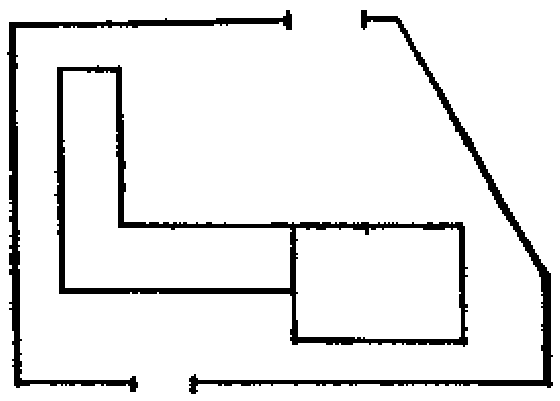
\includegraphics[width=6.0cm]{../pic/czjh1-ch5-xiti17-13.png}
    \caption*{(第 13 题)}
\end{figure}


\end{enhancedline}
\end{xiaotis}

